\section{W08 - Supply Chain Management}
\subsection{Introduction to SCM \index{Supply Chain Management}}
\subsubsection{The Revolution in 1983}
\subsubsection{Swatch 1992: 100’000’000 Uhr }
\subsubsection{Understanding the Impact of Supply Chain Disruptions}
\subsubsection{Supply Chain Glitches\index{Supply Chain!Glitch} Can Affect a Company’s Performance}
Auswirkung auf Aktienkurs be Lieferproblemen, x-Achse = 1 Jahr.\\
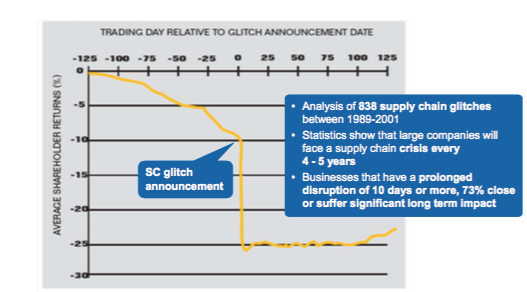
\includegraphics[width=1\textwidth]{W08/glitch}
\subsubsection{Comparison: The Effect of a Supply Chain Glitch	(-20\% to -25\% Stock Price Reduction)}
\begin{tabular}{|l|l|}
	\hline Statement & Stock Price Reaction \\ 
	\hline \multicolumn{2}{|c|}{ \textbf{Operations Events}}   \\ 
	\hline Increase in R\&D spending & 1.4\% \\ 
	\hline Closing factories & -0.7\% \\ 
	\hline Successful TQM & 0.6\%  \\ 
	\hline Successful green initiatives & 1.9\%  \\ 
	\hline  \multicolumn{2}{|c|}{ \textbf{Marketing Events}}    \\ 
	\hline Contracting of celebrities & 0.2\%  \\ 
	\hline Introduction of new product & 0.3\%  \\ 
	\hline  \multicolumn{2}{|c|}{ \textbf{IT}}    \\
	\hline  IT problems & -1.8\%  \\ 
	\hline 
\end{tabular} 
\subsubsection{Case Study: McDonalds Meat Scandal in China}
\subsubsection{Case Study: Toyota}
\subsubsection{Was Everything just a Misunderstanding? }
\subsubsection{Which Industries Are most Likely to Be Influenced by Supply Chain Glitches?}
\subsubsection{Supply Chain Management\index{Supply Chain!Management}:	From Sheep to Shawl}
\subsubsection{This is not Supply Chain Management – Optimizing yourself on	cost of other players in the chain}
! Just in Time  ist gef\"ahrlich!
spezialisierte Produkte die schnell ausgeliefert werden m\"ussen, brauchen hohe Lagerkosten. Auf keinen Fall zum externen Warenlager werden.
\subsubsection{Logistics = Supply Chain Management ?}
\subsubsection{Key Terminology of Supply Chain Management}
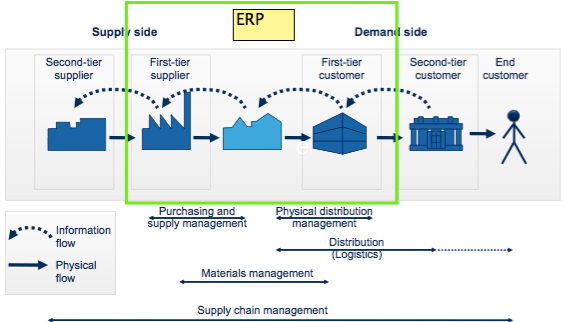
\includegraphics[width=1\textwidth]{W08/keyterm}
\subsection{Bullwhip Effect}
\subsubsection{The Bullwhip Effect: Increasing Variability Upstream\index{Upstream}}
1. F\"ur den Bullwhip Effect\index{Bullwhip!Effect} braucht es ''st\"orung'' in der Beschaffung (mehr Einkauf als geplant)\\
2. F\"ur Bullwhip Effect braucht es einen Zeitverzug zwischen Suppliers.
Um zu vermeiden -> alle in der Lieferkette m\"ussen informiert sein.
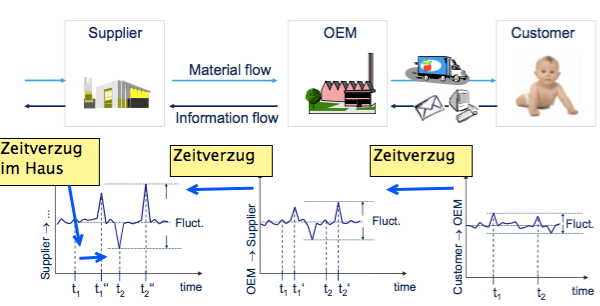
\includegraphics[width=1\textwidth]{W08/variabilityupstream}
\subsubsection{The Bullwhip Effect Can also Happen within a Company}
\subsubsection{Even Whole Economies Can Become Volatile: Machine Tools at the Tip of the Bullwhip}
\subsubsection{The Bullwhip Effect during the Financial Crisis in 2009}
\subsubsection{Impact of Bullwhip}
\index{Bullwhip!Impact}
\begin{enumerate}
\item High inventory
\item Out-of-stocks (OOS\index{OOS}) backlog cost
\item Low operational efficiency
\begin{itemize}
	\item underutilization
	\item overtime
	\item expediting
	\end{itemize}
\item Unnecessary capacity investment
\item Swings in working capital
\end{enumerate}
\subsubsection{What causes the Bullwhip Effect? 6 Main Reasons}
\begin{enumerate}
	\item Over-reaction to backlogs
	\item Neglecting to order based on inventory position
	\item Ordering in batches 
	\item Price variations (eq. Promotions)
	\item Lack of communication \& coordination - shortage gaming
	\item Delay times for information and delivery of materials
\item
\end{enumerate}
\subsubsection{Reducing the Price (Promotions) Creates Spikes}
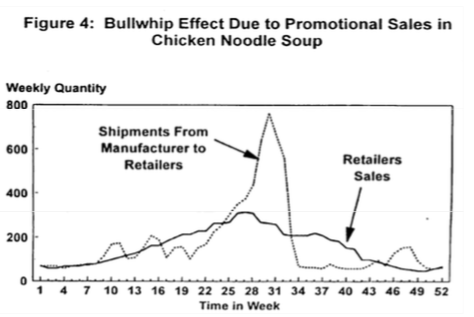
\includegraphics[width=1\textwidth]{W08/bullwhipnoodlesoup}
\subsubsection{``Chinese Whispers``: Information Distortion along the Supply Chain}
If one start to panic, all will start to panic. -> Domino
\subsubsection{How to Fight the Bullwhip Effect?}
\begin{enumerate}
	\item ERP-Systeme
	\item SCM-Systeme
	\item konstante Preise
	\item automatisierter Datenaustausch
	\item E-Commerce
	\item Vendor Managed Inventory
	\item automatisierte Bestellsysteme
\end{enumerate}
\subsubsection{ Automatic Replenishment Systems Can Mitigate the Effects of Overreaction}
\subsubsection{Eliminate Promotions with ``Every Day Low Prices`` (EDLP)}
\subsubsection{Handelsradar (Mai 2011) – Datenaustausch zwischen Industrie und Handel}
\subsubsection{Handelsradar Supply Side: Warum tauschen Sie nicht mehr	Daten aus?}
\subsubsection{Shorten Supply Chain: Let the Vendor Manage the Inventory}
\subsection{Designing the Supply Chain}
\subsubsection{Goals of Supply Chain Management}
\begin{itemize}
	\item Right quality: Every link is responsible for its own quality and that of its suppliers 
	\item High speed: The faster the throughput time, the more flexible	and cheaper the whole chain becomes 
	\item Reliability: Being on time, in full deliveries on all supply chain tiers 
	\item Flexibility: Supply chain agility is a prerequisite for reacting effectively to glitches and changes
	\item Cost: Reducing the overall transaction and transport costs of the whole chain
\end{itemize}
\subsubsection{How to design and optimize a Supply Network?}
\subsubsection{Choose the Right Supply Chain for each Product: Segmentation Logic by M. Fisher}
\subsubsection{Different Products Require Different Supply Chain Strategies}
